\chapter{Modified Fluid Closure}\label{chap:kinbrag}
This chapter puts together the pieces of the previous chapters in order to approximate a collisionless plasma with a modified fluid closure. The fastest-growing modes are shifted to longer wavelengths, and now instability requires
\begin{equation}
  \lambda^2>\frac{(2\pi v_A)^2}{3\Omega^2}\left(1+(p_\perp-p_\parallel)\frac{4\pi}{B^2}\right)
\end{equation}
As the instability grows, the fastest-growing modes may become larger than the simulation box size. \\
\\
Section~\ref{sec:athenamod} explains a modification to the Athena code introduced in Section~\ref{sec:codes}, while the next sections present the results of the pressure anisotropy both with and without limiters explained in Chapter~\ref{ssec:kinclosure}.

\section{Modification to Athena} \label{sec:athenamod}
The pressure anisotropy limiter was inserted manually into the code using the simplified version
\begin{align*}
  p_\perp-p_\parallel&<-\frac{B^2}{4\pi} & p_\perp-p_\parallel&>\frac{B^2}{8\pi}
\end{align*}
We shall see later if this assumption affects the results of the simulations.\\
\\
Since shearing-box simulations with anisotropic viscosity have never been done before, the publicly-available code did not work perfectly initially. The issue stemmed from using the orbital advection algorithm FARGO, which takes into account the background shear of a differentially-rotating disk to improve the efficiency and accuracy of the code. The code then solves for fluctuations on top of this background~\cite{Stone2010}.\\
\\
When the orbital advection algorithm is in use, the shear velocity needs to be removed from calculating the pressure anisotropy and viscous stress. The result is a simple insertion of an $if$ statement into various places in the code, but this change dramatically impacts the output variables since the pressure anisotropy depends on the gradient of the velocity. Without the modification, the pressure anisotropy $p_\perp-p_\parallel$ is negative, which makes no sense because the perpendicular pressure should grow with increasing magnetic field. However, such a mistake did reveal that the dominant pressure anisotropy is due to the background shear.
\begin{figure}[h!]
  \begin{center}  
    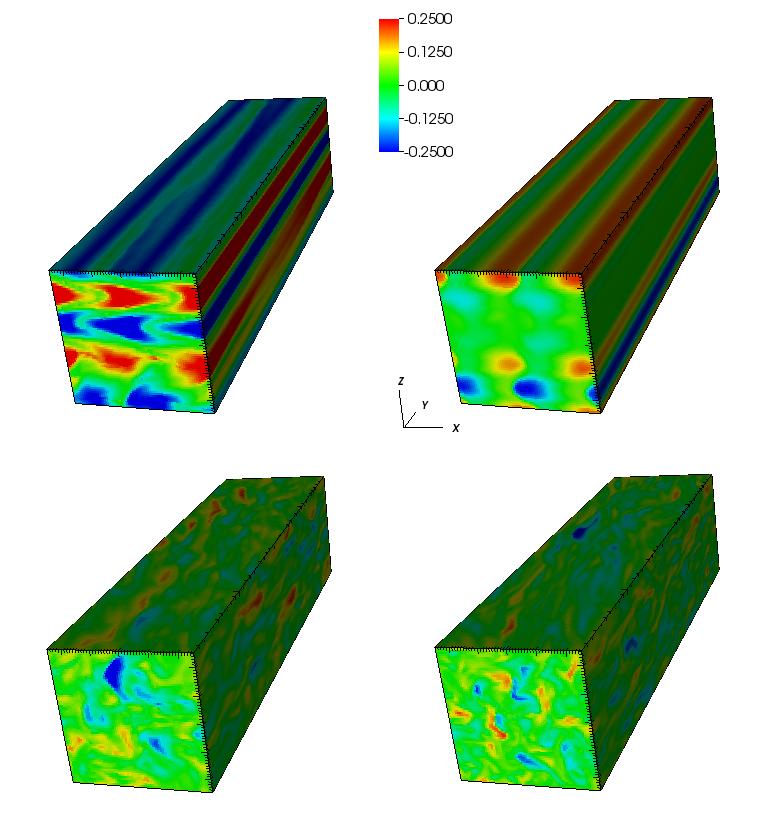
\includegraphics[width=.95\textwidth, angle=0.]{img/capped_uncapped_compare_dVy_t34t100.png}
  \end{center}
  \caption{Comparison of evolution of azimuthal angular momentum perturbations for uncapped (left) and capped (right) anisotropy. The top row is at time $t=3.4$ orbits and the bottom is at $t=10.0$ orbits.}
  \label{fig:vtkAn}
\end{figure}
\section{Linear Growth}
%
Although the main goal of this thesis is to characterize the nonlinear regime of turbulence, it is still useful to look at the linear growth of the MRI and compare the anisotropic limited and unlimited viscosity cases. Figure~\ref{fig:vtkAn} plots the azimuthal angular momentum perturbations at two different times for both cases. The limiter clearly affects the evolution of the turbulence, as shown by the top row, where the angular momentum perturbations saturate in the uncapped case. At the end of ten orbits, the turbulence in the uncapped case has larger patches of material that is moving in opposite direction. This effect will be discussed further in Section~\ref{sec:palim}.
%
%
\section{Comparison with Isotropic Viscosity}
%
%
\begin{figure}[h]
  \begin{center}  
    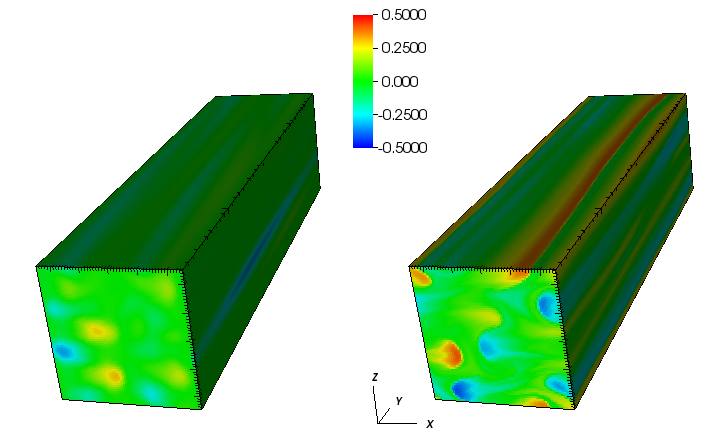
\includegraphics[width=.9\textwidth, angle=0.]{img/aniso_iso_compare_dVy_t35.png}
  \end{center}
  \caption{Short comparison of azimuthal angular momentum perturbations at $t=3.5$ orbits for isotropic viscosity (left) and capped pressure anisotropy (right). }
  \label{fig:vtkcompare}
\end{figure}

%
%
%-----------------------------------------------------------------------------------------
%
Comparing the anisotropic viscosity to the well-understood isotropic viscosity case discussed in Chapter~\ref{chap:compMRI} shows the complexity of anisotropic viscosity. Figure~\ref{fig:vtkcompare} shows the entire shearing box domain for isotropic and anisotropic viscosity. When anisotropic viscosity is enabled, the transport properties are altered, as evidence by the different shapes of the modes.\\
\\
Figure~\ref{fig:eta1Pm4All} compares different box-averaged quantities for isotropic viscosity and the two types of anisotropic viscosity. The isotropic viscosity magnetic energy thrives as discussed in Chapter~\ref{sec:localnonideal}. The channel mode is evident in all three cases and the relative importance of the different $x$, $y$, and $z$ components also remains the same. The uncapped anisotropic viscosity, however, decays in magnetic energy while the other two grow or remain more-or-less constant. Whether a dynamo is present actually remains to be seen, since these simulations were only run for 10 orbits whereas typical simulations to determine if the dynamo is sustained run for on the order of 100 orbits. It is possible that the magnetic energy for the anisotropic viscosity will rebound. If it does not, then we must explain why the uncapped pressure anisotropy decays in magnetic energy.\\
\\
\begin{figure}[H]
  \begin{center}  
    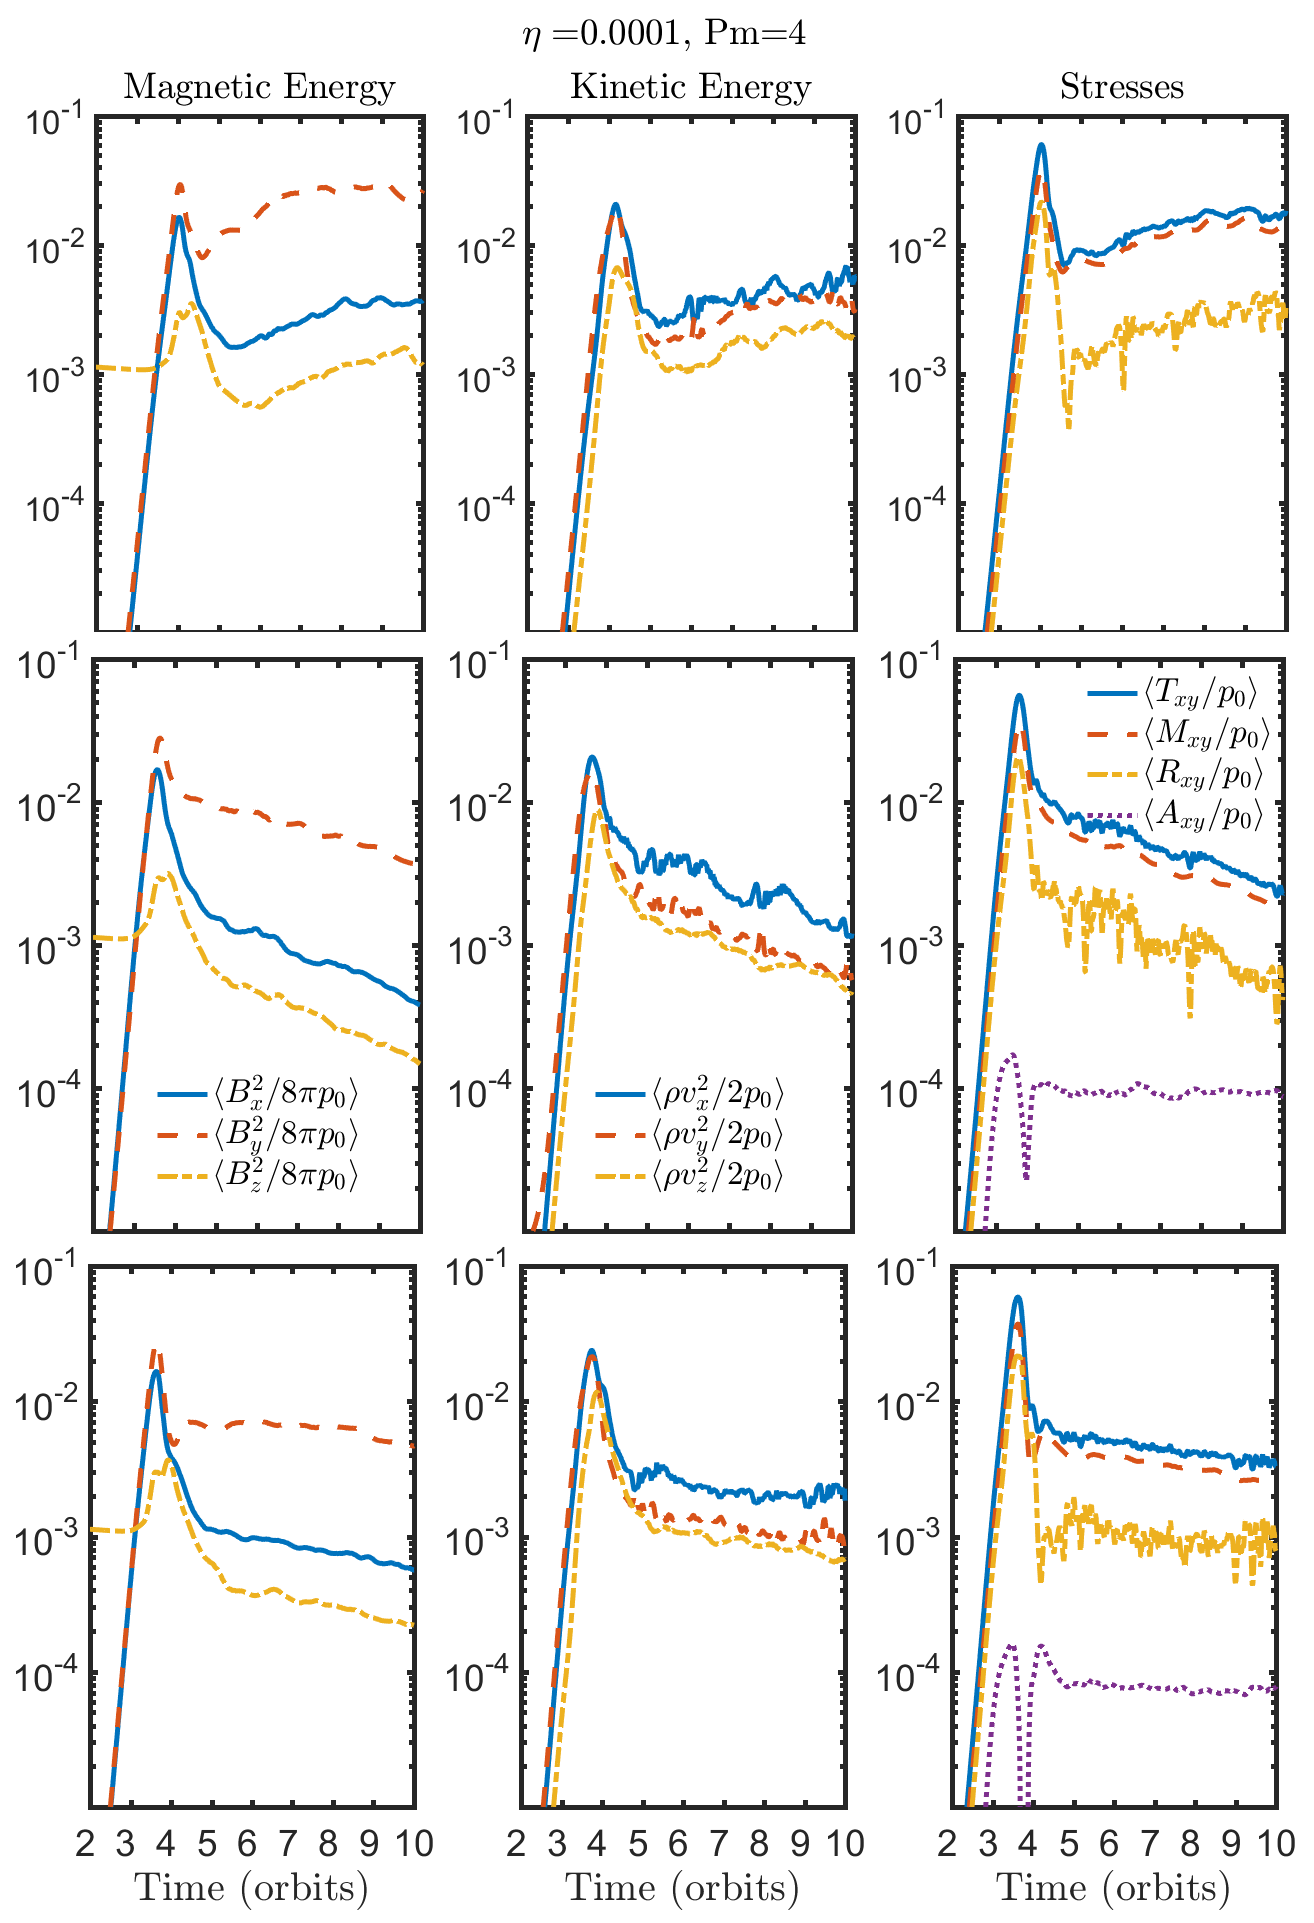
\includegraphics[width=.95\textwidth, angle=0.]{img/eta1-Pm4-All.png}
  \end{center}
  \caption{Comparison of three types of viscosity: isotropic (top), anisotropic uncapped (middle), and anisotropic capped (bottom).}
  \label{fig:eta1Pm4All}
\end{figure}
%
\noindent If we think about anisotropic viscosity as viscosity that only acts along the magnetic field lines, then it is effectively one-third the isotropic value. Thus an isotropic magnetic Prandtl number of 4 would mean an effective magnetic Prandtl number of $4/3$ in the anisotropic case. We could therefore be running into the problems of minimum (or ``critical'') $Pm$ discussed in Chapter~\ref{chap:compMRI}. Simulations with larger box size would be able to tell.\\
\\
The difference between unlimited and limited pressure anisotropy can be readily explained. The anisotropy limiter keeps dissipation in check, whereas in the uncapped case it increases uncontrollably and therefore damps the magnetic activity. The same is true for kinetic energy. These results suggest that the values of $\eta=\num{1e-4}$ and $\nu=\num{4e-4}$ are appropriate for studying sustained turbulence in the anisotropy-limited case.\\
\\
The stresses involved are important because the viscous stress $A_{xy}=-(p_\perp-p_\parallel)\frac{B_xB_y}{B^2}$ is what gives rise to increased angular momentum transport~\cite{Kunz2016}. Figure~\ref{fig:eta1Pm4All} shows that the evolution of the total stress $T_{xy}$ in all three cases is dominated by the Maxwell stress $M_{xy}=-\frac{B_xB_y}{4\pi}$, while the Reynolds stress $R_{xy}=\rho u_xu_y$ is about an order of magnitude lower. These values are about an order of magnitude lower than in~\citetalias{Kunz2016}, most likely due to the value of the transport coefficients. Clearly, the viscous stress with these values barely plays a role, whereas in~\citetalias{Kunz2016} the viscous stress is slightly below but comparable to the Maxwell stress. In order to better replicate~\citetalias{Kunz2016}, we need higher values of viscosity.\\
\\
Figure~\ref{fig:eta1Pm150} accordingly shows a higher value of $\nu$ for the capped and uncapped anisotropic viscosity (the isotropic viscosity's magnetic energy decays, not shown). However, both because the viscosity is only acting along one direction and the fastest-growing mode is at larger wavelengths, the magnetic energy for the anisotropic viscosity does not decay, as indicated by the flat Maxwell stress in both the capped and uncapped case. However, the viscous stress fails to surpass the Reynolds stress in terms of importance. We can attempt to fix this by looking at higher values of resistivity and viscosity.%\\
%\\
\begin{figure}[H]
  \begin{center}  
    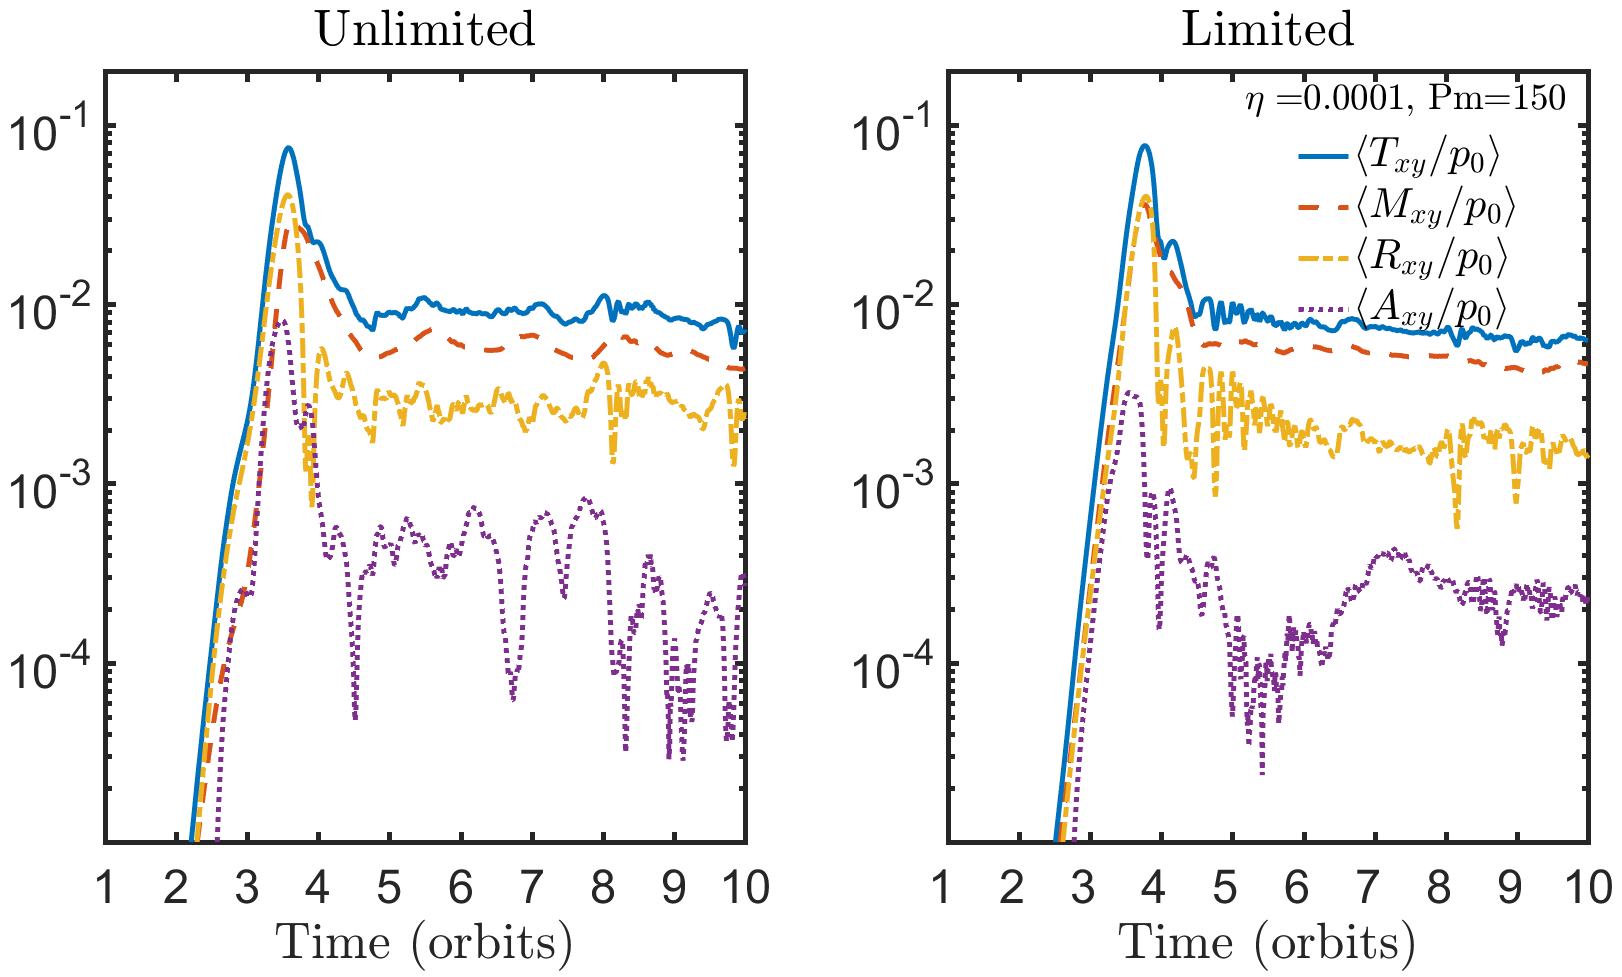
\includegraphics[width=\textwidth, angle=0.]{img/eta1-Pm150-Stresses-Abs.png}
  \end{center}
  \caption{Comparison of limited and unlimited anisotropic viscosity stresses at high values of $\nu$: here, $\nu=\num{1.5e-2}$.}
  \label{fig:eta1Pm150}
\end{figure}
%
\noindent Figure~\ref{fig:eta2Pm150} shows an equivalent $Pm$ of 150 but with the resistivity increased by a factor of two. As seen in the unlimited case, the viscous stress now rises to approximately the same order of magnitude as the Reynolds and Maxwell stress. However, the magnetic energy is decreasing in both cases, as seen by the downward-sloping Maxwell stress which of course limits the viscous stress for the capped anisotropy case. Unfortunately, higher resistivity appears not to sustain turbulence, which is needed for the MRI to transport angular momentum. The effect is even more dramatic at higher resistivity. We therefore need to keep looking at lower resistivities but at higher viscosity. \\
\\
For reference and comparison to Fig. 11 in~\citet{Fromang2007b}, we plot whether the magnetic energy is clearly sustained, clearly decays, or somewhere in-between (to be established with longer simulations) as a function of Reynolds number and magnetic Reynolds number in Figure~\ref{fig:fromangPlot}. Results are also summarized in Table~\ref{tab:etapmturb}.\\
\\
%
\begin{figure}[H]
  \begin{center}  
    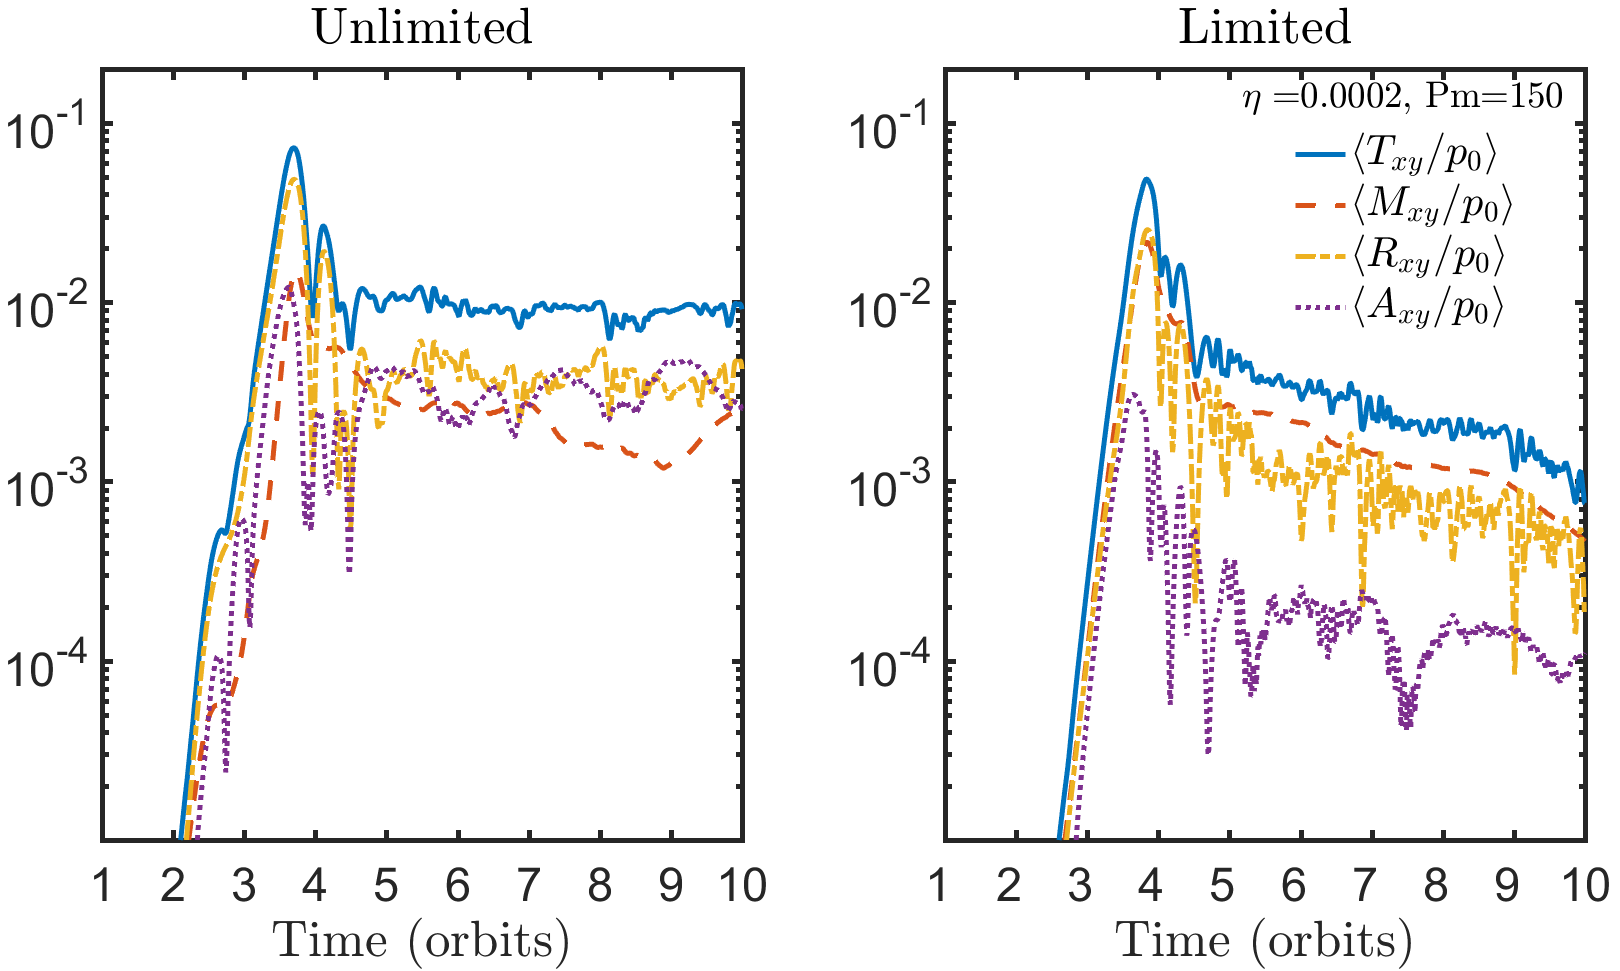
\includegraphics[width=\textwidth, angle=0.]{img/eta2-Pm150-Stresses-Abs.png}
  \end{center}
  \caption{Comparison of limited and unlimited anisotropic viscosity stresses at a higher value of $\eta$: here, $\eta=\num{2e-4}$.}
  \label{fig:eta2Pm150}
\end{figure}
%
\begin{table}[H]
  \centering
  \begin{tabular}{c|c|c|c|c|c|c|c|c|c|c|c|c|c}
    $\eta$/$Pm$ &4&6&8&12&16&20&24&30&40&50&75&100&150 \\\hline
    \num{1e-4} &Y&Y&Y&?&Y&?&?&Y&?&Y&?&?&Y\\\hline
    \num{2e-4} &Y&?&N&Y&Y&?&Y&?&N&N&N&N&N\\\hline
    \num{3e-4} &N&N&?&N&N&N&Y&?&N&?&?&N&N\\\hline
    \num{4e-4} &N&N&N&N&N&N&N&N&N&N&N&N&?
  \end{tabular}
  \caption{Display of trials run and whether the magnetic energy is sustained (Y), decays (N), or is unclear (?), necessitating longer trials.}
  \label{tab:etapmturb}
\end{table}
%
\begin{figure}[h]
  \begin{center}  
    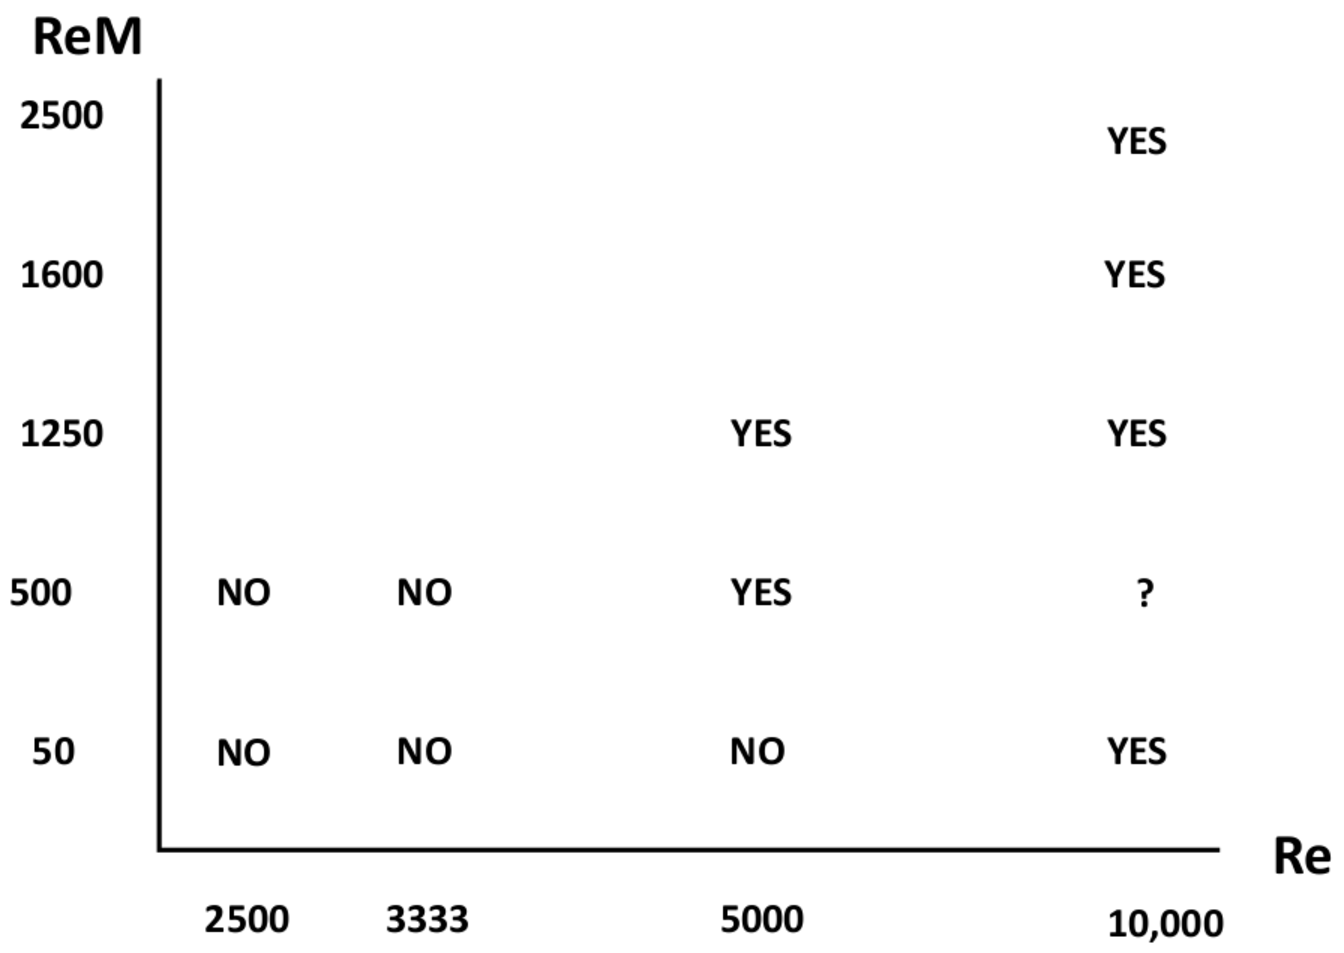
\includegraphics[width=\textwidth, angle=0.]{img/fromangPlot.pdf}
  \end{center}
  \caption{Summary of capped anisotropic viscosity's ability to sustain magnetic energy and hence turbulence, necessary for accretion. The question mark means that it is difficult to tell whether the dynamo is sustained without longer trial runs. Complements~\citet{Fromang2007b}.}
  \label{fig:fromangPlot}
\end{figure}
\noindent The next section will look at the distinguishing feature of the anisotropic viscosity, the pressure anisotropy, and analyze how the limiter behaves.

%--------------------------------------------------------------------------%
\section{Effect of the Pressure Anisotropy Limiter}\label{sec:palim}
\begin{figure}[h]
  \begin{center}  
    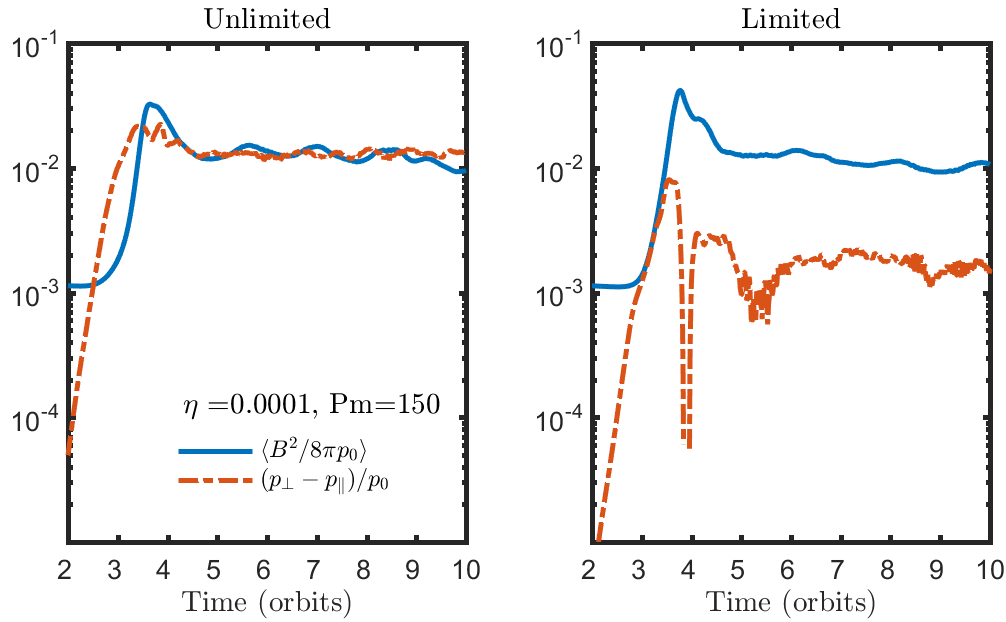
\includegraphics[width=\textwidth, angle=0.]{img/eta1-Pm150-PAME.png}
  \end{center}
  \caption{Comparison of unlimited and limited anisotropic pressure time evolution, with magnetic energy plotted for reference.}
  \label{fig:eta1Pm150PAME}
\end{figure}
%
\begin{figure}[h]
  \begin{center}  
    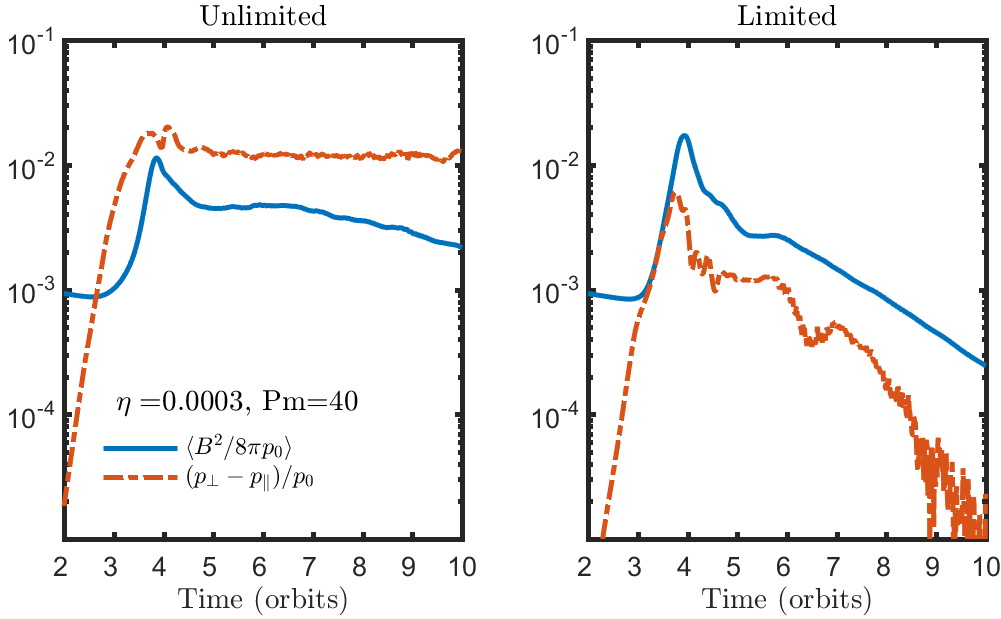
\includegraphics[width=\textwidth, angle=0.]{img/eta3-Pm40-PAME.png}
  \end{center}
  \caption{Comparison of unlimited and limited anisotropic pressure time evolution, with magnetic energy plotted for reference.}
  \label{fig:eta3Pm40PAME}
\end{figure}
%
\begin{figure}[h]
  \begin{center}  
    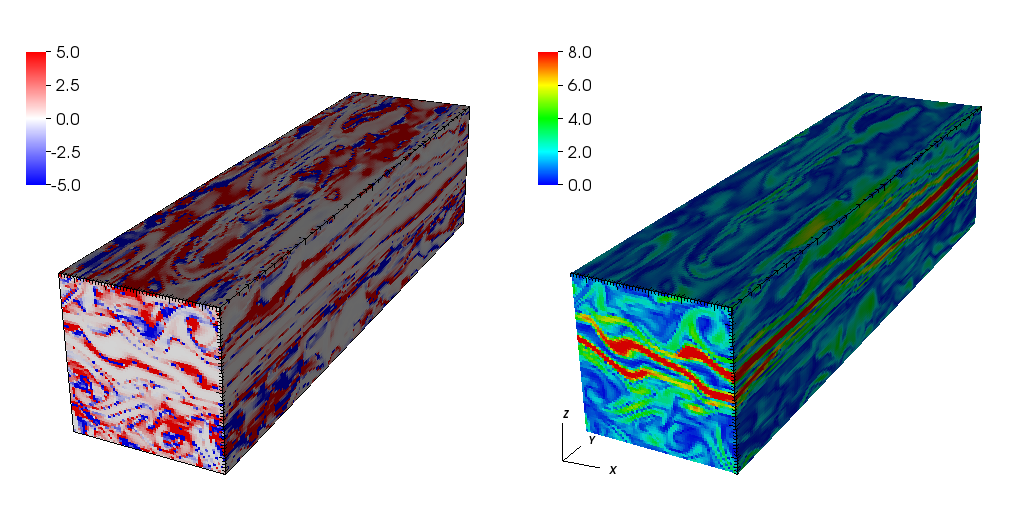
\includegraphics[width=\textwidth, angle=0.]{img/yca-eta1R1L1-13-PA-t41.png}
  \end{center}
  \caption{Anisotropy-limited shearing box domain during the nonlinear regime at $t=4.1$ orbits. Left: the pressure anisotropy $p_\perp-p_\parallel$ normalized to initial pressure. Right: magnetic field strength magnitude, normalized to initial field strength.}
  \label{fig:vtkPA}
\end{figure}
%
\begin{figure}[h]
  \begin{center}  
    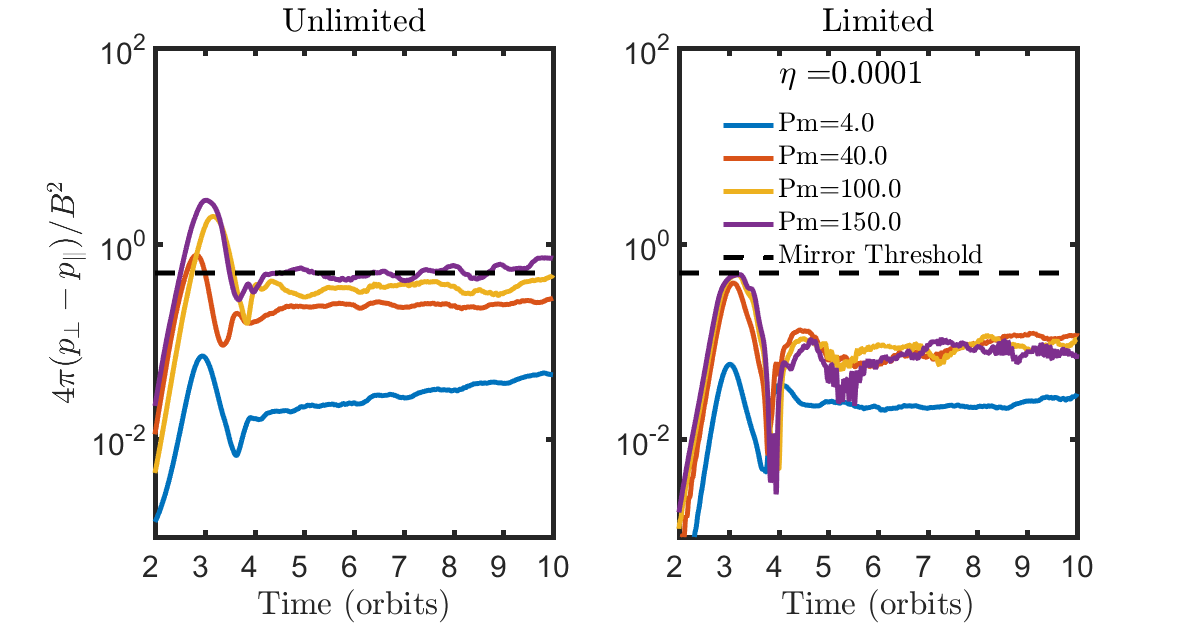
\includegraphics[width=\textwidth, angle=0.]{img/eta1-Pm4-40-100-150-PAMElog.png}
  \end{center}
  \caption{Pressure anisotropy normalized to magnetic energy, which makes it clear when the mirror threshold (dashed line) is exceeded.}
  \label{fig:eta1PAMElog}
\end{figure}
%
\begin{figure}[h]
  \begin{center}  
    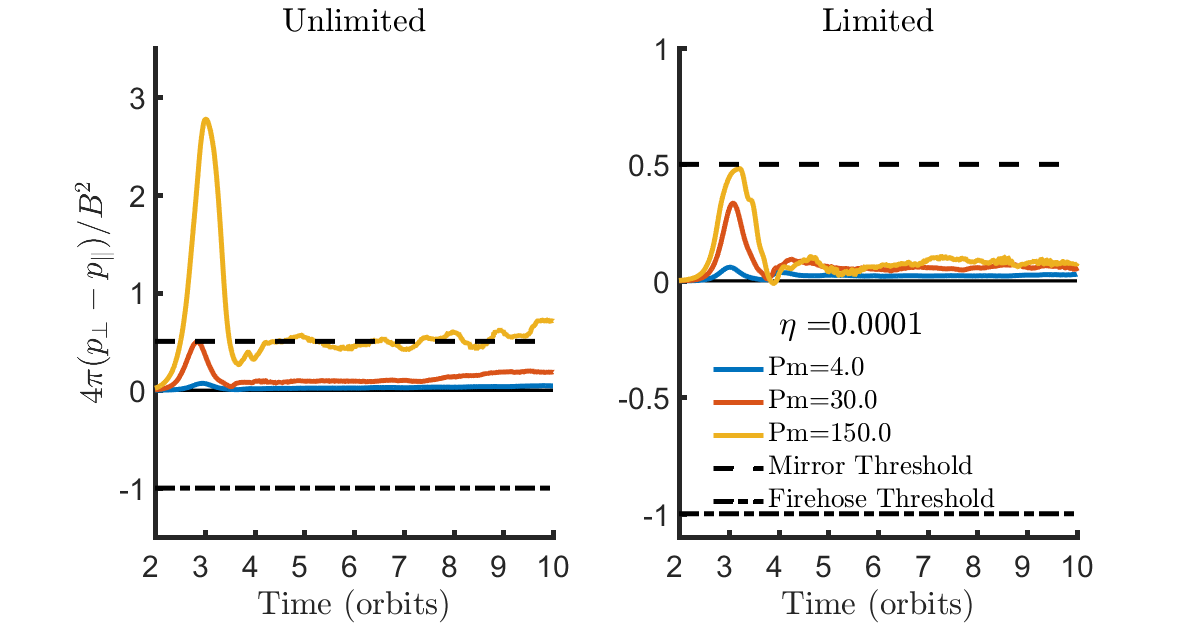
\includegraphics[width=\textwidth, angle=0.]{img/eta1-Pm4-30-150-PA.png}
  \end{center}
  \caption{Pressure anisotropy normalized to magnetic energy, showing how the lower firehose threshold is never violated.}
  \label{fig:eta1PAME}
\end{figure}
%
%------------------------------------------------------------------------------------------------------
%
The main goal of the pressure anisotropy limiter was to prevent the anisotropy from increasing beyond the mirror threshold. We can see the effect in Figure~\ref{fig:eta1Pm150PAME}. The unlimited case has an anisotropy that exceeds the magnetic energy at early times and over the course of its evolution. The anisotropy stays around a constant value, as in~\citetalias{Sharma2006}'s run in Figure 5. Although there are several differences between this simulation and the one in~\citetalias{Sharma2006} (including net flux, equation of state, and exact bounds for the mirror instability), the idea is the same. The pressure anisotropy saturates, just like the magnetic energy. \\
\\
Higher values of viscosity and resistivity exhibit the same saturation of the pressure anisotropy as seen in Figure~\ref{fig:eta3Pm40PAME}. However, in these cases the magnetic energy decays as discussed above, which significantly impacts the anisotropy-limited case but not the unlimited case. This is interesting because decreasing magnetic energy leads to an increase in parallel pressure, so even in the unlimited case one might expect to see the pressure anisotropy decrease with decreasing magnetic energy. However, since the goal of this thesis requires magnetic energy to be sustained, we shall not delve into this issue further. It might simply be a question of running the simulation for longer, since the effect is slight.\\
\\
It is reassuring to see in both Figure~\ref{fig:eta1Pm150PAME} and Figure~\ref{fig:eta3Pm40PAME} that the pressure anisotropy bumps right up against the mirror threshold (which is the magnetic energy, plotted in solid blue) during the first few orbits. The limiter is clearly having an effect on the anisotropy value. However, as the unlimited case demonstrates, right before the channel phase is the main time when the limiter is important. This justifies our simplifying use of $\beta_\parallel$ instead of $\beta_\perp$ in the limiter equation because the two are roughly equal at that point in the evolution.\\
\\
As the magnetic energy begins decreasing after the end of the channel mode, the anisotropy no longer adheres strictly to the limiter. This is because the pressure anisotropy is a volume averaged-quantity. As the magnetic field decreases, the parallel pressure increases since $p_\parallel B^2\sim const$. In some places of the computational domain, the pressure anisotropy is negative; that is, the pressure along the magnetic field lines exceeds the pressure perpendicular to the field lines. This can be seen explicitly in Figure~\ref{fig:vtkPA}, which plots the approximate pressure anisotropy throughout the domain. The fact that the pressure anisotropy is not only positive means that the volume-averaged value will be lower than the positive-definite magnetic energy and hence there is a gap between the lines in Figures~\ref{fig:eta1Pm150PAME} and~\ref{fig:eta3Pm40PAME}. \\
\\
We can see the effect of the anisotropy limiter across magnetic Prandtl number in Figure~\ref{fig:eta1PAMElog}, which plots selected magnetic Prandlt numbers for $\eta=\num{1e-4}$. All trials plotted have sustained magnetic energy. As already noted, lower values of viscosity do not hit the mirror threshold, whereas the effects become clearer at higher values. Larger values of resistivity exceed the mirror threshold earlier.\\
\\
For completeness, Figure~\ref{fig:eta1PAME} shows another set of magnetic Prandtl number, demonstrating that the firehose threshold never comes into play. This is expected since the magnetic energy grows due to the MRI, and $p_\perp\sim B$. However, in trials with higher resistivity and high magnetic Prandtl number (not shown), the pressure anisotropy seems to dip slightly negative. This is probably due to the magnetic energy not being sustained and thus $p_\parallel$ increasing, but it is still worth pursuing. 




